\chapter*{Le crêpier psycho-rigide}

À la fin de sa journée, un crêpier dispose d'une pile de crêpes désordonnée. Le
crêpier étant un peu psycho-rigide, il décide de ranger sa pile de crêpes, de la
plus grande (en bas) à la plus petite (en haut), avec le coté brûlé caché.

\begin{center}
  \begin{frame}{Activité: Le crêpier psycho-rigide}

  \begin{block}{Matériel}
    \begin{itemize}
    \item des planchettes en bois de tailles et de couleurs différentes (faces reconnaissables)
    \item éventuellement une pelle à tarte pour retourner les planchettes
    \end{itemize}
  \end{block}

  \begin{block}{Règle du jeu}
    \begin{itemize}
      \item \structure{Installation :} Faire une pile désordonnée de crêpes.
      \item \structure{Objectif :} ranger les crêpes de la plus grande (en bas) à la plus petite (au haut), face colorée vers le haut.
      \item \structure{Coup autorisé :} prendre une ou plusieurs crêpes sur le haut de la pile, et de les reposer à l'envers.
    \end{itemize}
  \end{block}

  \bigskip \bigskip \bigskip

  \begin{center}
    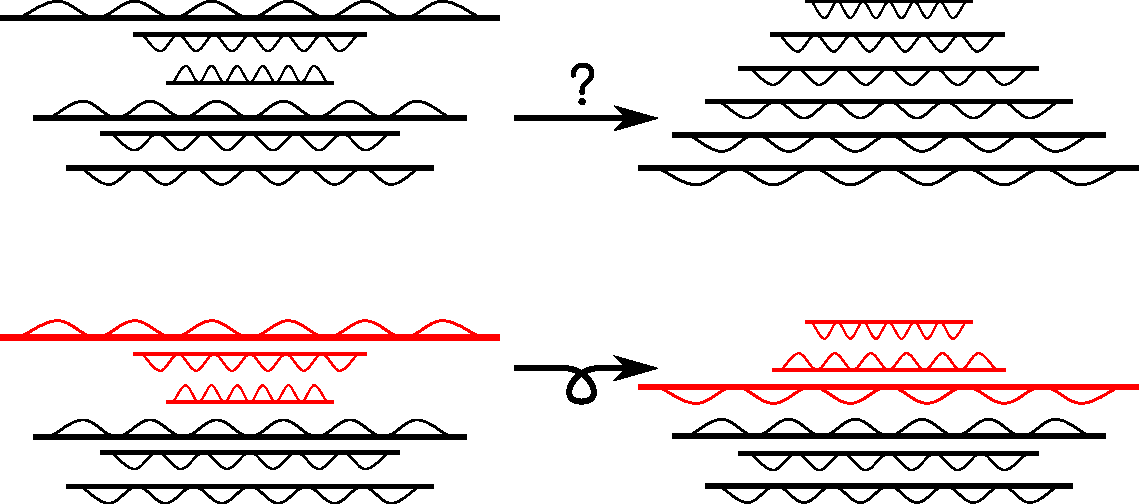
\includegraphics[width=0.8\linewidth]{img/crepier.pdf}
  \end{center}

\end{frame}

\begin{frame}{Ce qu'il faut retenir du  crêpier psycho-rigide}

  \begin{columns}
    \begin{column}{.7\linewidth}
      \begin{block}{Un algorithme}
        \begin{itemize}
        \item n'a d'intérêt que si on peut l'expliquer
        \item doit être suffisamment simple pour pouvoir l'expliquer à une machine
        \item \alert{\textbf{«Diviser pour mieux régner»}} : on essaie toujours de décomposer un algorithme en tâches simples
        \end{itemize}
      \end{block}

      \begin{block}{L'algorithme que doit suivre le crêpier est :}
        \begin{itemize}
        \item ramener la plus grande crêpe en haut de la pile
        \item retourner pour que la face brûlée soit vers le haut
        \item retourner la pile de sorte à mettre la plus grande crêpe en bas
        \item réitérer avec la crêpe de taille inférieure
        \end{itemize}
      \end{block}

      \begin{block}{Le rapport avec l'informatique}
        \begin{itemize}
        \item l'informaticien passe son temps à trouver des algorithmes et  à les expliquer à la machine
        \item le principe \alert{\textbf{«Diviser pour mieux régner»}} est fondamental en informatique
        \end{itemize}
      \end{block}
    \end{column}

    \begin{column}{.3\linewidth}
      \begin{block}{Pour aller plus loin}
        Selon l'état initial de la pile de crêpes, le nombre minimum de coups nécessaires pour la ranger varie.

        \begin{itemize}
          \item Quel est le meilleur état initial possible (qui demandera le moins de coups pour ranger) ?
          \item Quel est le pire état initial possible ?
          \item Combien faut-il de coups pour ranger une pile de $N$ crêpes dans le pire des cas ?
        \end{itemize}
      \end{block}
    \end{column}
  \end{columns}
      
\end{frame}

\begin{frame}{Ce qu'il faut retenir du crêpier psycho-rigide : performance d'algorithmes}

  \begin{block}{Pourquoi évaluer la performance d'un algorithme ?}

    Évaluer la performance d'un algorithme nous permet :

    \begin{itemize}
      \item de se faire une idée du temps nécessaire pour résoudre un problème de plus grande taille (combien de temps pour un million de crêpes ?) ;
      \item de le comparer à d'autres aglorithmes résolvant le même problème, pour savoir lequel est le meilleur.
    \end{itemize}

  \end{block}

  \begin{block}{Comment évaluer la performance d'un algorithme ?}

    \begin{itemize}
      \item On compte le nombre de coups nécessaires dans le cas général. Pour le crêpier :
        \begin{itemize}
          \item pour ranger une crêpe, il faut entre $0$ coups (la crêpe est déjà rangée) et $3$ coups (amener en haut, retourner, amener à sa place) ;
          \item pour $n$ crêpes (cas général), il faut entre $0$ et $3 \times n$ coups ;
          \item la performance d'un algorithme sur un cas particulier dépend donc beaucoup de l'état initial, mais en règle générale on s'intéresse surtout aux cas intermédiaires, qui sont les plus probables.
        \end{itemize}
      \item $n$ est une variable qui exprime la taille du problème. La performance d'un algorithme est notée comme une fonction de la taille du problème nommée $O$.
      \item La performance exprime un ordre de grandeur plutôt qu'une évaluation précise du temps d'exécution. Pour des grandes valeurs de $n$, il n'est pas très utile de faire la distinction entre $O(n)$, $O(n+4)$ ou encore $O(3 \times n)$ - surtout quand on compare avec un autre algorithme dont la performance est $O(n^2)$. 
      \item On simplifie donc en retirant les constantes pour ne garder que les termes les plus importants. Pour le crêpier, on notera la performance de notre algorithme $O(n)$ ; on dit alors que le temps de calcul croit \textit{linéairement} avec $n$. En revanche, un algorithme $O(n^2)$ aurait une croissance \textit{quadratique}, et un algorithme $O(2^n)$ aurait une croissance \textit{exponentielle}.
     \end{itemize}
  \end{block}

  \begin{block}{À la recherche du meilleur algorithme possible}
    \begin{itemize}
    \item On arrive parfois à montrer qu'on a le meilleur algorithme possible. Par exemple on ne peut pas trier les éléments en moins de $n$ étapes, car on doit forcément tous les considérer.
    \item On peut aussi prouver qu'un tri comparatif ne peut pas se faire en moins de $n\times log(n)$ étapes, car il n'accumule pas assez d'information pour choisir la bonne permutation en moins d'étapes.
    \item Mais la plupart du temps, on ne sait pas prouver que l'algorithme connu est le meilleur possible. C'est alors le meilleur \textit{connu}, sans être forcément le meilleur \textit{possible}.
    \end{itemize}
  \end{block}

  %\begin{block}{À la recherche de problèmes difficiles}
    %\begin{itemize}
    %\item On peut classifier les problèmes en fonction de la performance des algorithmes les résolvant. \\
      %(cela permet de se forger un sens commun de ce qui est faisable avec un ordinateur et éviter les problèmes si difficiles qu'ils sont quasi impossibles)
    %\item Il existe énormément de problèmes relativement simples pour lesquels personne ne connaît de bon algorithme, sans que personne n'arrive non plus à démontrer qu'un tel algorithme n'existe pas.
    %\item L'activité suivante sera l'occasion d'explorer un peu cette classification des problèmes très durs.
    %\end{itemize}
  %\end{block}
\end{frame}

\end{center}

Pour cette tâche, le crêpier peut faire une seule action : glisser sa spatule
entre deux crêpes et retourner le haut de la pile. Comment doit-il procéder pour
trier toute la pile ?

\begin{center}
  \newcommand{\crepe}[5]{ % size yshift xshift flip
	\draw [color=#5, dashed, thick, yshift=#2*0.4cm, xshift=#3cm,rotate=#4*180] (-#1,0.1) -- (#1,0.1);
	\draw [color=#5, thick, yshift=#2*0.4cm, xshift=#3cm,rotate=#4*180](-#1,0.1) -- (-#1,-0.1) -- (#1,-0.1) -- (#1,0.1);
}

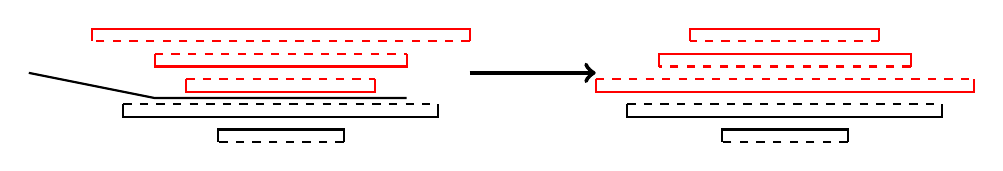
\begin{tikzpicture}[scale=0.8]

% \crepe{1cm}{0}{180};
% \crepe{1.5cm}{(0,1.5)}{0};
% \crepe{2cm}{(0,0)}{180};
% \crepe{2.5cm}{(0,1)}{0};
% \crepe{3cm}{(0,2)}{0};

\crepe{3cm}{4}{0}{1}{red};
\crepe{2cm}{3}{0}{0}{red};
\crepe{1.5cm}{2}{0}{0}{red};

% dessin de la pelle à tarte (une pelle à crêpes, ça n'existe pas ?)
\draw [color=black, thick, yshift=2*0.4cm, xshift=0cm,rotate=0*180] (-4,0.2) -- (-2,-0.2) -- (2,-0.2);

\crepe{2.5cm}{1}{0}{0}{black};
\crepe{1cm}{0}{0}{1}{black};

\draw [->,ultra thick,draw] (3,1) -- (5,1) ;

\crepe{1.5cm}{4}{8}{1}{red};
\crepe{2cm}{3}{8}{1}{red};
\crepe{3cm}{2}{8}{0}{red};
\crepe{2.5cm}{1}{8}{0}{black};
\crepe{1cm}{0}{8}{1}{black};


\end{tikzpicture}

\end{center}

\encart{Matériel}{
  \begin{itemize}
  \item Des planchettes en bois de tailles et de couleurs différentes (faces
    reconnaissables)
  \item Une pelle à tarte pour retourner les planchettes (optionnelle)
  \end{itemize}
}

%\begin{center}
  %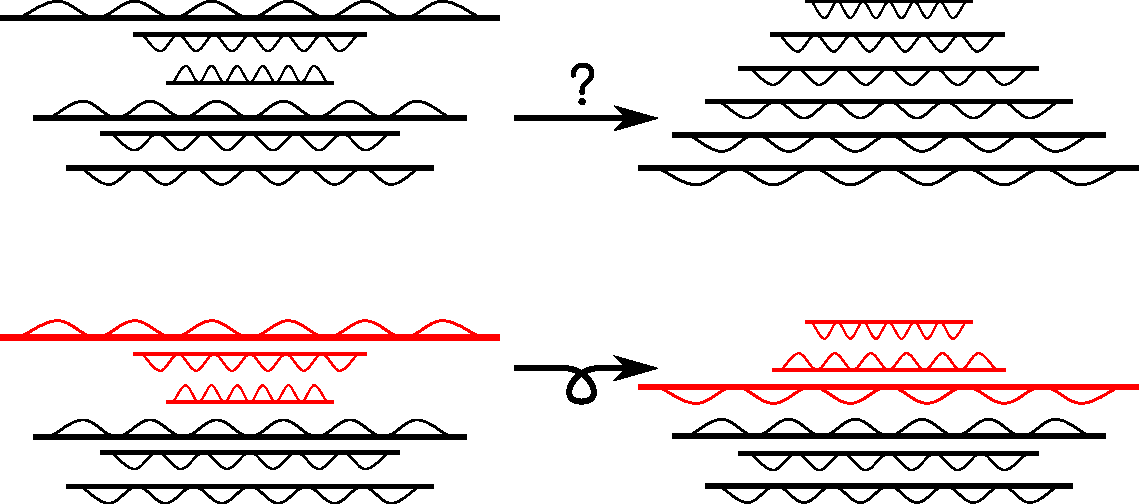
\includegraphics[width=0.6\linewidth]{img/crepier.pdf}
%\end{center}

\newpage

\section*{Description d'un algorithme}

L'algorithme permettant de résoudre le problème du crêpier est le suivant :

\begin{enumerate}
\item amener la plus grande crêpe en haut de la pile
\item mettre la face brûlée vers le haut
\item retourner toute la pile - la crêpe est rangée
\item recommencer en ignorant les crêpes rangées
\end{enumerate}

Cet algorithme assez simple nous apprend deux choses. Premièrement, un
algorithme n'a d'intérêt que si on peut l'expliquer - pire encore, que si on
peut l'\textit{expliquer à un ordinateur}. Il doit donc être \textbf{écrit sans
  ambiguïté}. Deuxièmement, un algorithme décompose le problème en une série de
tâches simples. On appelle ce principe \textbf{\og Diviser pour mieux
  régner\fg}.

Ce que nous venons de décrire est le c\oe{}ur de métier des informaticiens:
analyser un problème, le subdiviser en problèmes plus simples, formaliser le
tout sous la forme d'un algorithme, et traduire l'algorithme dans un langage
compréhensible par l'ordinateur.

\section*{Performance d'un algorithme}

Le premier objectif de l'écriture d'un algorithme est qu'il résolve le
problème. Le second objectif est qu'il le résolve le plus vite possible.

Évaluer la \textbf{performance d'un algorithme} nous permet de nous faire une
idée du temps nécessaire à la résolution d'un problème de grande taille. Par
exemple, combien de temps faudra-t-il à notre algorithme pour trier une pile
d'un million de crêpes ?

De plus, s'il existe plusieurs algorithmes résolvant le même problème,
l'évaluation de la performance nous donne un critère objectif pour savoir lequel
est le plus efficace.

\subsection*{Évaluer la performance d'un algorithme}

Pour évaluer la performance, on compte le nombre de \og coups \fg\ nécessaires
pour résoudre le problème dans le cas général. Pour le problème du crêpier :

\begin{itemize}
\item pour ranger une crêpe, il faut entre $0$ coup (la crêpe est déjà rangée)
  et $3$ coups (amener en haut, retourner, amener à sa place) ;
\item pour $n$ crêpes (cas général), il faut entre $0$ coup (meilleure
  situation) et $3 \times n$ coups (pire situation). La performance de
  l'algorithme dépend donc beaucoup de l'état initial, mais on s'intéresse
  surtout aux cas intermédiaires, qui sont les plus probables.
\end{itemize}

Ici, $n$ est une variable qui exprime la taille du problème. La performance d'un
algorithme est notée comme une fonction de la taille du problème nommée
$O$. Pour le crêpier, on peut donc écrire $O(3 \times n)$.

Le temps d'exécution variant selon l'état initial, la performance exprime
l'ordre de grandeur du temps d'exécution. Pour des grandes valeurs de $n$, il
n'est pas très utile de faire la distinction entre $O(n)$, $O(n+4)$ ou encore
$O(3 \times n)$ --- en particulier quand on compare avec un autre algorithme
dont la performance est $O(n^2)$.

On simplifie donc en retirant les constantes pour ne garder que les termes
importants. Pour le crêpier, on notera donc la performance de notre algorithme
$O(n)$ ; on dit alors que la performance de l'algorithme est \textit{linéaire},
car le temps de calcul croît linéairement avec $n$. Un algorithme avec une
performance $O(n^2)$ est dit \textit{quadratique}, tandis qu'un algorithme
$O(2^n)$ est dit \textit{exponentiel}.

\subsection*{À la recherche du meilleur algorithme possible}

On arrive parfois à montrer qu'on a le meilleur algorithme possible. Par
exemple, on ne peut pas trier les éléments en moins de $n$ étapes, car on doit
forcément tous les considérer.

On peut aussi prouver qu'un tri comparatif ne peut pas se faire en moins de
$n\times log(n)$ étapes, car il n'accumule pas assez d'informations pour choisir
la bonne permutation en moins d'étapes.

Mais la plupart du temps, on ne sait pas prouver que l'algorithme connu est le
meilleur possible. C'est alors le meilleur \textit{connu}, sans être forcément
le meilleur \textit{possible}.
    
\section*{Le coin de l'animateur}

L'objectif de cette activité est de trouver un algorithme, de le faire
verbaliser par les participants et d'en mesurer la performance.

\begin{itemize}
\item Expliquez les règles et demandez aux participants de tenter de résoudre le
  problème ;
\item s'ils bloquent, conseillez-les. Par exemple : \og essaye d'abord de mettre
  la grande crêpe en bas \fg, ou encore \og où doit se trouver la grande crêpe
  pour pouvoir l'amener en bas ? \fg
\item Quand les participants ont trouvé l'algorithme, demandez-leur de
  l'expliquer.
\item Demandez ensuite de calculer le nombre de coups nécessaires pour ranger la
  pile de crêpes. Le nombre de coups dépendant de l'état initial, faites-les
  généraliser en trouvant le nombre de coups maximal pour ranger une crêpe, puis
  $n$ crêpes.
\item Le discours sur le $O(n)$ est volontairement approximatif. On veut faire
  sentir les choses; faire un vrai cours prend une douzaine d'heures
  (cf. \url{http://www.loria.fr/~quinson/Teaching/TOP/}).
  % \item Au passage, le crêpier ne ressemble pas du tout aux tours de Hanoï:
  %   l'histoire ressemble un peu, mais la résolution est très différente (il y
  %   a $2^n-1$ étapes à Hanoï et $3\times n$ au crêpier).
\end{itemize}


